\documentclass[tikz,border=4pt]{standalone}
\usepackage{pgfplots}
\pgfplotsset{compat=1.18}

\begin{document}
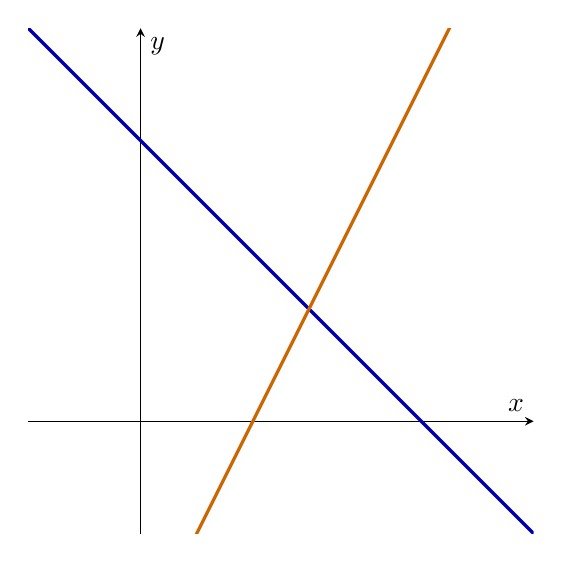
\begin{tikzpicture}
\begin{axis}[
    axis lines=center,
    xlabel={$x$},
    ylabel={$y$},
    xmin=-2, xmax=7,
    ymin=-2, ymax=7,
    xtick=\empty, ytick=\empty,
    width=8cm, height=8cm,
    clip=true
]

% Line 1: y = -x + 5 (blue)
\addplot[domain=-2:7, samples=2, very thick, blue!70!black] {-x + 5};

% Line 2: y = 2x - 4 (orange)
\addplot[domain=-2:7, samples=2, very thick, orange!80!black] {2*x - 4};

\end{axis}
\end{tikzpicture}
\end{document}
